\PassOptionsToPackage{sols}{handout}
\documentclass[main]{subfiles}
\setcounterrefbeforedot{chapter}{m-ws6-5}
\setcounterrefafterdot{section}{m-ws6-5}
\addtocounter{section}{-1}
\usepackage{solutions}

\begin{document}

\ifSubfilesClassLoaded{%
  \chaptermark{\chaptersix}
}{}

\section{Slicing to Find Area} \label{ws6-5}

\begin{problemonly}
    \begin{framed}

\textbf{Key Ideas}:

\begin{itemize}[topsep=0pt,partopsep=0pt,parsep=8pt,itemsep=0pt]


\item You should be able to write a Riemann sum that approximates the area
  between multiple curves, as well as a definite integral that gives the
  \emph{exact} area.

\item You should be comfortable with our process for finding such areas:
  \textbf{slice} the region either vertically or horizontally,
  \textbf{approximate} the area of a typical slice by pretending that it's
  a rectangle, \textbf{sum} to get a Riemann sum approximation for the
  entire area, and \textbf{take a limit} to get a definite integral giving
  the exact area. 

\item You should be able to find the area of a region by slicing
  vertically or horizontally, and you should be able to decide which
  method is more useful in a given situation.  (This may involve some
  trial and error; if the first way you slice is not helpful, try the
  other way!)

\item You should appreciate that there are times when a definite integral
  can be computed more easily by visualizing it as an area and slicing the
  area horizontally rather than vertically.


\end{itemize}
\end{framed}
\end{problemonly}

\begin{enumerate}
\item The tide removes sand from a certain beach at 
a rate modeled by the function
$R(t)=2+5\sin\Bigl(\dfrac{\pi t}{6}\Bigr).$
A machine adds sand to the beach at a rate modeled by
the function
$S(t)=\dfrac{18t}{5+3t}.$

Both $R(t)$ and $S(t)$ have units of cubic meters per hour, and $t$
is measured in hours for $0 \leq t \leq 6$. At time $t=0$, the beach contains $3000$ cubic meters of sand. 
\begin{enumerate}
    \item Explain the meaning of the following values in this context.
    \emph{(Think about the units.)}

    \begin{enumerate}
        \item \begin{problem}[\vfill]
        $R(1)=4.5$
        \end{problem}

        \begin{solution}
            At $t=1$, the rate at
            which the tide removes sand from the beach is
            $4.5$ cubic meters per hour.
        \end{solution}
        
        \item \begin{problem}[\vfill]
        $S(1)=2.25$
        \end{problem}

        \begin{solution}
            At $t=1$, the rate at which the machine adds sand to the beach is $2.25$ cubic meters
            per hour.
        \end{solution}
        
        \item \begin{problem}[\vfill] 
        $S(1)-R(1)=-2.25$
        \end{problem}

        \begin{solution}
            At $t=1$, the rate of
            change of the total amount of sand on the beach is
            $-2.25$ cubic meters per hour, i.e. the amount of sand
            is decreasing at a rate of $2.25$ cubic meters per hour.
        \end{solution}

    \end{enumerate}

    
    \item \begin{problem}[\vfill]
    Write an expression for $f(t)$, the rate of change
    of the total amount of sand on the beach in cubic meters per hour
    at time $t$.
    \end{problem}

    \begin{solution}
        The rate of change of the total amount of sand on the beach
        is the rate at which sand is added to the beach minus the 
        rate at which sand is removed from the beach,
        \[f(t)=\left(\text{rate in}\right) - 
        \left(\text{rate out}\right) = 
        \boxed{S(t)-R(t).}\]
    \end{solution}
        \pspace{16pt}
        
    \item \begin{problem}[\vfill\newpage]
        Write an expression for $M(t)$, the total number of
    cubic meters of sand on the beach at time $t$.
    \end{problem}

    \begin{solution}
        Since the rate of change of the total amount of sand
        on the beach is $S(t)-R(t)$ and the amount of sand on the
        beach at $t=0$ is $3000$ cubic meters, 
        \[M(t)=\boxed{3000+\int_0^t \bigl(S(x)-R(x)\bigr)dx.}\]
    \end{solution}
    \pspace{16pt}
    \end{enumerate}
    Use the graphs of $R$ and $S$ shown below to answer the following
    parts.
    
    \probonly{\begin{minipage}[t]{0.4\textwidth}}
    \begin{center}
    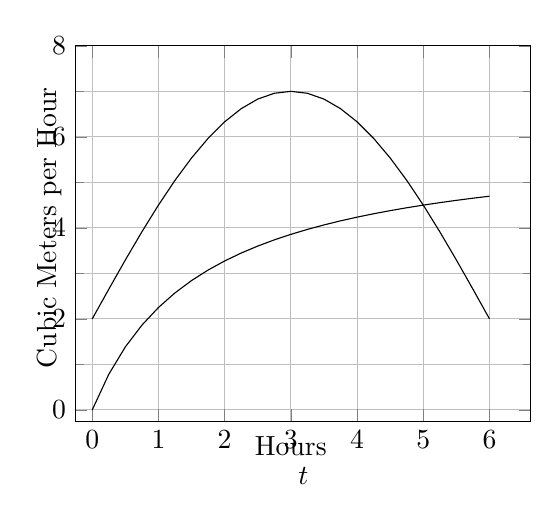
\begin{tikzpicture}
        \begin{axis}[xmin=-0.25, ymin = -0.25, ymax=8,
        minor y tick num = 1, xtick distance = 1,
        grid=both, xlabel=$t$, clip=false, height = 2.5in]
            \node at (3,-0.8) {Hours};
            \node[rotate=90] at (-0.65,4) {Cubic Meters per Hour}; 
            \addplot[domain=0:6]{2+5*sin(deg(pi*x/6))};
            \addplot[domain=0:6]{18*x/(5+3*x)};
        \end{axis}
    \end{tikzpicture}
    \end{center}
    \probonly{\end{minipage}}
    \probonly{\begin{minipage}[t]{0.54\textwidth}}
    \begin{enumerate}[resume,topsep=0pt]
    \item Find the time interval(s) during which the total amount of
    sand on the beach is decreasing. 
    
        \begin{solution}
            $M(t)$ is
            decreasing when $M'(t)$ is negative. $M'(t)=S(t)-R(t)$.
            Looking at the graphs, we can see that $R(t)\geq S(t)$ on 
            the interval $[0,5]$ since the graph of $R$ crosses
            above the graph of $S$, so $M'(t)$ will be negative when
            $t<5$. 
            
            Therefore
            $M(t)$ is decreasing on the interval $\boxed{[0,5].}$
        \end{solution}

    \pspace{12pt}

    \item A beachgoer looks at this graph and determines that
    the total amount of sand on the beach is decreasing most rapidly
    at $t=3$. Are they correct? Explain.

    \begin{solution}
        The total amount of sand is decreasing most rapidly
        when $M'(t)$ is the most negative, i.e. when
        $R(t)-S(t)$ is largest. Looking at the graph, this actually
        between $t=2$ and $t=3$, at around $t\approx2.6$, since
        that is where the distance between the graphs is the largest.
        
        At $t=3$, $R(t)$ is at a maximum, which means that this is when sand is being removed most rapidly. But this does not
        take into account the rate at which sand is being added to the
        beach. So the beachgoer is \fbox{not correct.}

    \begin{center}
    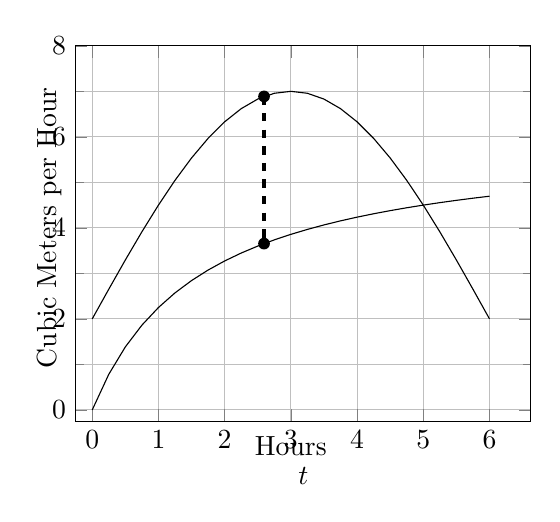
\begin{tikzpicture}
        \begin{axis}[xmin=-0.25, ymin = -0.25, ymax=8,
        minor y tick num = 1, xtick distance = 1,
        grid=both, xlabel=$t$, clip=false, height = 2.5in]
            \node at (3,-0.8) {Hours};
            \node[rotate=90] at (-0.65,4) {Cubic Meters per Hour}; 
            \addplot[domain=0:6]{2+5*sin(deg(pi*x/6))};
            \addplot[domain=0:6]{18*x/(5+3*x)};
            \coordinate (A) at (2.595,6.888);
            \coordinate (B) at (2.595,3.654);
            \draw[very thick, dashed] (A) -- (B);
            \draw[radius=2pt] (A) node[circle,fill,inner sep=1.5pt] {}
            (B) node[circle,fill,inner sep=1.5pt] {};
        \end{axis}
    \end{tikzpicture}
    \end{center}
    \end{solution}

    
    \end{enumerate}
        \probonly{\end{minipage}}
    \begin{enumerate}[start=7]
    \item \begin{problem}[\vfill] 
    At what time $t$ is the total
    amount of sand least? Justify your answer.
    \end{problem}

    \begin{solution}
        Since $M(t)$ is decreasing on the interval $[0,5]$ and
        increasing on the interval $[5,6]$, the minimum amount of
        sand occurs at time $\boxed{t=5.}$
    \end{solution}

    \item \begin{problem}[\vfill]
    At what time $t$ is the total
    amount of sand greatest? Justify your answer.
    \end{problem}
    
    \begin{solution}
        The critical points of $M(t)$ are at $t=0$, $5$, and $6$.
        From the reasoning in part (g), we know that $M(t)$ 
        attains its minimum at $t=5$. This leaves two candidates for
        the maximum, $t=0$ and $t=6$. 
        
        Looking at the graph, we can
        see that the net change from $t=0$ to $t=6$, 
        $\displaystyle\int_0^6 \bigl(S(t)-R(t)\bigr)dt$, 
        is negative. Thus, the maximum amount of sand occurs
        at time $\boxed{t=0.}$
    \end{solution}

    
    \item \begin{problem}[\vfill]
    What does $\displaystyle\int_0^5 \bigl(R(t)-S(t)\bigr)dt$
    mean in this context? What does it represent graphically?
    \end{problem}

    \begin{solution}
        $\displaystyle\int_0^5\bigl(S(t)-R(t)\bigr)dt$ is the
        net change in the amount of sand from $t=0$ to $t=5$. This
        is negative since between $t=0$ and $t=5$, more sand 
        is removed than is added. Since
        \[\int_0^5 \bigl(R(t)-S(t)\bigr)dt 
        = -\int_0^5 \bigl(S(t)-R(t)\bigr)dt,\]
        $\displaystyle\int_0^5 \bigl(R(t)-S(t)\bigr)dt$
        will have the same magnitude but will be positive. It 
        represents the decrease in the amount of sand between $t=0$
        and $t=5$.

        Graphically, this integral represents the area of the 
        region bounded
        by the $y$-axis and the graphs of $y=R(x)$ and $y=S(x)$ as
        shown.
        

    \begin{center}
    \begin{tikzpicture}
        \begin{axis}[xmin=-1, xmax = 7, ymin = -3, ymax=8,
        height = 2.5in]
            \addplot[domain=-1:7]{2+5*sin(deg(pi*x/6))};
            \addplot[domain=-1:7]{18*x/(5+3*x)};
            \addplot[name path=R,domain=0:5]{2+5*sin(deg(pi*x/6))};
            \addplot[name path=S,domain=0:5]{18*x/(5+3*x)};
            \draw[black, thick] (0,0) -- (0,2);
            \addplot[blue!50,opacity=0.5] fill between[of=R and S];
        \end{axis}
    \end{tikzpicture}
    \end{center}
    \end{solution}
\end{enumerate}

\pspace{\newpage}

\item 
  \note{The parabola here crosses the $x$-axis, so this is a good place to
    talk about the fact that the principle ``vertical distance = (top
    $y$-coordinate) - (bottom $y$-coordinate)'' always applies, even when
    the bottom $y$-coordinate is negative.

    If you like, you can have students first try this problem by adding up
    signed areas (like ``area under $e^x$ from $x = 1$ to $x = 3$'' minus
    ``area under $x^2 - 4$ from $x = 2$ to $x = 3$'' + ``negative of the
    signed area under $x^2 - 4$ from $x = 1$ to $x = 2$'').  

    It's probably also worth pointing out that we're now talking about
    plain old (positive) area, not signed area.
  }

  \begin{problem}[0.75in]
    Find the area under $y = e^x$, above $y = x^2 - 4$, to the right of $x
    = 1$, and to the left of $x = 3$.

    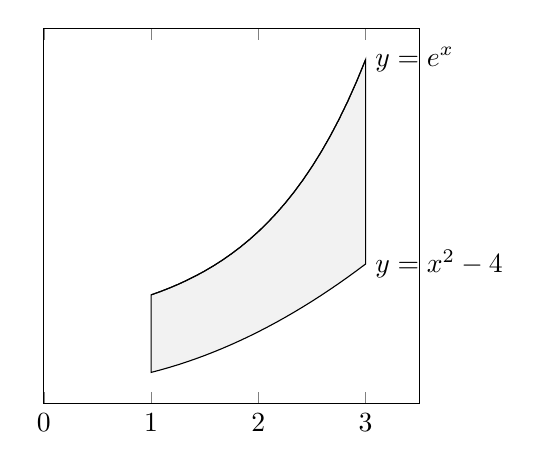
\begin{tikzpicture} 
      \begin{axis}[stack plots=y, cycle list={black}, xmin=0, xmax=3.5, 
        width=2.5in, height=2.5in, clip=false, ytick=\empty] 
        \addplot+[domain=1:3]{e^x} node [right] {$y = e^x$}; 
        \addplot+[domain=1:3, fill=lightgray, fill opacity=0.2] 
        {x^2-4-e^x} \closedcycle; 
        \node [right] at (axis cs: 3, 5) {$y = x^2 - 4$}; 
      \end{axis} 
    \end{tikzpicture}
  \end{problem}

  \begin{solution}
    We \textbf{slice} the interval $[1, 3]$ into $n$ pieces of equal width
    $\Delta x$, label $x_0 = 1, \ldots, x_n = 3$ as usual, and focus on
    the $k$-th slice.  We can approximate this slice as a rectangle:
    \begin{center}
      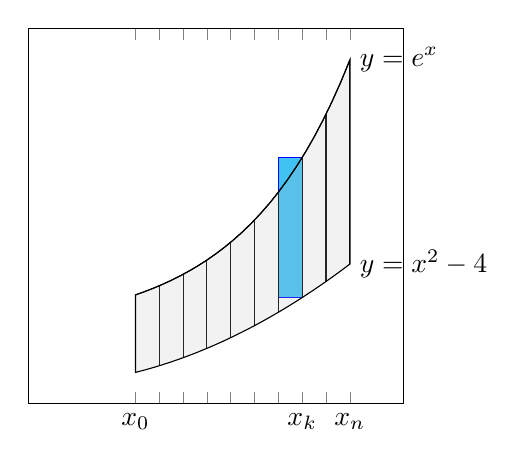
\begin{tikzpicture}[declare function={f(\x)=e^\x; g(\x)=\x^2-4;}]
        \begin{axis}[stack plots=y, cycle list={black}, xmin=0, xmax=3.5, 
          width=2.5in, height=2.5in, clip=false, xtick={1, 1.222, ...,
            3.01}, xticklabels={$x_0$, , , , , , , $x_k$, , $x_n$},
          disabledatascaling, ytick=\empty]  
          \addplot+[domain=1:3]{e^x} node [right] {$y = e^x$}; %
          \addplot+[domain=1:3, fill=lightgray, fill opacity=0.2]
          {x^2-4-e^x} \closedcycle; %
          \node [right] at (axis cs: 3, 5) {$y = x^2 - 4$}; %
          \pgfplotsforeachungrouped \x in {1, 1.222, ..., 3.01}
          {
            \pgfmathsetmacro{\y}{f(\x)}
            \pgfmathsetmacro{\z}{g(\x)}
            \edef\temp{%
              \noexpand\draw (\x, \y) -- (\x, \z);
            }
            \temp
          }          
          \draw[fill=cyan, fill opacity=0.75, draw=blue] (2.333, {f(2.555)})
          -- (2.555, {f(2.555)}) -- (2.555, {g(2.555)}) -- (2.333,
          {g(2.555)}) -- (2.333, {f(2.555)}); %
        \end{axis}
      \end{tikzpicture}
    \end{center}
    The rectangle has height (top $y$-coordinate) $-$ (bottom
    $y$-coordinate) $=$ $e^{x_k} - (x_k^2 - 4)$ and width $\Delta x$,
    so
    \[ \text{area of $k$-th slice} \approx \left[ e^{x_k} - (x_k^2 - 4)
    \right] \Delta x.\]
    Summing up the areas of all the slices,
    \[ \text{area of region} \approx \sum_{k=1}^n \left[ e^{x_k} - (x_k^2 - 4)
    \right] \Delta x.\]
    Taking the limit as $n \to \infty$ (that is, as the number of slices
    increases without bound),
    \begin{align*}
      \text{area of region} &= \int_1^3 \left[ e^x - (x^2 - 4) \right]
      dx \\
      &= \int_1^3 \left( e^x - x^2 + 4 \right) dx \\
      &= \left. e^x - \frac{x^3}{3} + 4x \right|_1^3 \\
      &= \left( e^3 - 9 + 12 \right) - \left( e - \frac{1}{3} + 4 \right)
      \\
      &= \boxed{e^3 - e - \frac{2}{3}}
    \end{align*}
  \end{solution}

\item 
  \note{The main new thing here is that they need to figure out which
    curve is on top, and they also need to solve for the endpoints of
    integration.} 

  \begin{problem}[\vfill]
    Find the area of the region bounded by $y = 2 - x^2$ and $y = x$.
  \end{problem}

  \begin{solution}
    Here is the region in question:
    \begin{center}
      \begin{tikzpicture}
        \begin{axis}[disabledatascaling, cycle list name=mycolor, cycle
          list shift=1]
          \addplot+[domain=-2:1, fillregion, draw=none] {2-x^2} -- (-2,
          -2);
          \addplot+[domain=-2.25:2.25] {2-x^2};
          \addplot+[domain=-2.25:2.25] {x};          
        \end{axis}
      \end{tikzpicture}
    \end{center}
    First, let's figure out where the two curves intersect.  This happens
    where $2 - x^2 = x$, so let's start by solving that equation:
    \begin{align*}
      2 - x^2 &= x \\
      0 &= x^2 + x - 2 \\
      0 &= (x + 2)(x - 1)       
    \end{align*}
    So, the two curves intersect where $x = -2$ and $x = 1$.  Let's slice
    the region into $n$ vertical slices of equal thickness $\Delta x$,
    label $x_0 = -2, \ldots, x_n = 1$ as usual, and approximate the $k$-th
    slice by a rectangle:
    \begin{center}
      \begin{tikzpicture}[declare function={f(\t)=2-(\t)^2; g(\t)=\t;}]
        \begin{axis}[disabledatascaling, cycle list name=mycolor, cycle
          list shift=1, 
          xtick={-2, -1.72727, ..., 1.01}, ytick=\empty,
          xticklabels={$x_0$,,,,,,$x_k$,,,,,$x_n$}]
          \addplot+[domain=-2:1, fillregion, draw=none] {2-x^2} -- (-2,
          -2);
          \addplot+[domain=-2.25:2.25] {2-x^2};
          \addplot+[domain=-2.25:2.25] {x};          
          \pgfplotsforeachungrouped \x in {-2, -1.72727, ..., 1.01}
          {
            \pgfmathsetmacro{\y}{f(\x)}
            \pgfmathsetmacro{\z}{g(\x)}
            \edef\temp{%
              \noexpand\draw (\x, \y) -- (\x, \z);
            }
            \temp
          }
          \draw[blue, fill=cyan, fill opacity=0.75] (-0.6364,
          f{(-0.3636)}) -- (-0.3636, f{(-0.3636)}) -- (-0.3636,
          g{(-0.3636)}) -- (-0.6364, g{(-0.3636)}) -- cycle;
        \end{axis}
      \end{tikzpicture}
    \end{center}
    Therefore,
    \[ \text{area of $k$-th slice} \approx \left[ \left(2 - x_k^2 \right)
      - x_k \right] \Delta x,\] so the area of the region is
    \begin{align*}
      \int_{-2}^1 [(2 - x^2) - x]\,dx &= \int_{-2}^1 (2 - x^2 + x)\,dx \\
      &= \left. 2x - \frac{x^3}{3} + \frac{x^2}{2} \right|_{-2}^1 \\
      &= \left( 2 - \frac{1}{3} + \frac{1}{2} \right) - \left( -4 +
        \frac{8}{3} + 2 \right) \\
      &= \boxed{\frac{9}{2}}
    \end{align*}
  \end{solution}       

  % \item Find the area of the region in the first quadrant bounded by $y = \arcsin x, y = 
  %   \pi/2$, and $x=0$.

  %   

\item 
  \note{It's slightly more efficient to do this by slicing horizontally.} 

  \begin{problem}[\vfill\newpage]
    Find the area enclosed by $y = -2x$, $y = x^3$, and $y = 1$.
  \end{problem}

  \begin{solution}
    Let's draw a picture so we can see what area we're talking about.  If
    we graph $y = -2x$, $y = x^3$, and $y = 1$, we see that the area we're
    talking about is this:    
    \begin{center}
      \begin{tikzpicture}
        \begin{axis}[ymin=-1, ymax=1.75, width=2.5in, height=2.5in, cycle
          list name=mycolor, cycle list shift=2, clip=false, ytick={1}]
          \addplot+[domain=0:1, fillregion, draw=none] {x^3} -- (-0.5, 1)
          -- (0, 0);
          \addplot+[domain=-0.875:0.5] {-2*x} node[pos=0, above] {$y = -2x$};
          \addplot+[domain=-1:1.75^(1/3)] {x^3} node[right]{$y = x^3$};
          \addplot+[domain=-1.25:1.25] {1} node[right]{$y = 1$};
        \end{axis}
      \end{tikzpicture}
    \end{center}
    As always, the first step is to \textbf{slice}.  We can either slice
    horizontally or vertically: 
    \begin{center}
      \begin{tikzpicture}
        \begin{axis}[ymin=-1, ymax=1.75, width=2.5in, height=2.5in, cycle
          list name=mycolor, cycle list shift=2, clip=false, ytick={1},
          fixed point arithmetic]
          \addplot+[domain=0:1, fillregion, draw=none] {x^3} -- (-0.5, 1)
          -- (0, 0);
          \addplot+[domain=-0.875:0.5] {-2*x} node[pos=0, above] {$y = -2x$};
          \addplot+[domain=-1:1.75^(1/3)] {x^3} node[right]{$y = x^3$};
          \addplot+[domain=-1.25:1.25] {1} node[right]{$y = 1$};
          \pgfplotsforeachungrouped \y in {0.142857, 0.285714, ..., 1.01}
          {
            \edef\temp{%
              \noexpand\draw (-\y/2, \y) -- ({\y^(1/3)}, \y);
            }
            \temp
          }
        \end{axis}
      \end{tikzpicture}
      \hspace{0.5in}
      \begin{tikzpicture}
        \begin{axis}[ymin=-1, ymax=1.75, width=2.5in, height=2.5in, cycle
          list name=mycolor, cycle list shift=2, clip=false, ytick={1}]
          \addplot+[domain=0:1, fillregion, draw=none] {x^3} -- (-0.5, 1)
          -- (0, 0);
          \addplot+[domain=-0.875:0.5] {-2*x} node[pos=0, above] {$y = -2x$};
          \addplot+[domain=-1:1.75^(1/3)] {x^3} node[right]{$y = x^3$};
          \addplot+[domain=-1.25:1.25] {1} node[right]{$y = 1$};
          \pgfplotsforeachungrouped \x in {-0.5, -0.4, ..., 1.01}
          {
            \edef\temp{%
              \noexpand\draw (\x, {max(-2*\x, \x^3)}) -- (\x, 1);
            }
            \temp
          }
        \end{axis}
      \end{tikzpicture}      
    \end{center}
    Notice that, if we use vertical slices, there are two ``types'' of
    slices --- slices to the left of the $x$-axis go between the curves $y
    = -2x$ and $y = 1$ while slices to the right of the $x$-axis go
    between $y = x^3$ and $y = 1$.  This means we need to consider these
    two regions separately.

    If we use horizontal slices, then all of the slices have the same
    description: the left side is on $y = -2x$, and the right side is on
    $y = x^3$.  So, using horizontal slices is slightly more efficient.
    Therefore, we'll slice $[0, 1]$ into $n$ pieces, label $y_0 = 0,
    \ldots, y_n = 1$ as usual, and approximate the $k$-th slice as a
    rectangle:
    \begin{center}
      \begin{tikzpicture}
        \begin{axis}[ymin=-1, ymax=1.75, width=2.5in, height=2.5in, cycle
          list name=mycolor, cycle list shift=2, clip=false, ytick={0,
            0.142857, ..., 1}, yticklabels={$y_0$,,,,$y_k$,,,},
          fixed point arithmetic]
          \addplot+[domain=0:1, fillregion, draw=none] {x^3} -- (-0.5, 1)
          -- (0, 0);
          \addplot+[domain=-0.875:0.5] {-2*x} node[pos=0, above] {$y = -2x$};
          \addplot+[domain=-1:1.75^(1/3)] {x^3} node[right]{$y = x^3$};
          \addplot+[domain=-1.25:1.25] {1} node[right]{$y = 1$};
          \pgfplotsforeachungrouped \y in {0.142857, 0.285714, ..., 1.01}
          {
            \edef\temp{%
              \noexpand\draw (-\y/2, \y) -- ({\y^(1/3)}, \y);
            }
            \temp
          }
          \draw[blue, fill=cyan, fill opacity=0.75] (-0.285714,
            0.571429) -- ({0.571429^(1/3)}, 0.571429) --
            ({0.571429^(1/3)}, 0.428571) -- (-0.285714, 0.428571) -- cycle;
        \end{axis}
      \end{tikzpicture}      
    \end{center}
    This rectangle has height $\Delta y$, and its width is (right
    $x$-coordinate) $-$ (left $x$-coordinate).  The right side is on the
    curve $y = x^3$, or $x = y^{1/3}$; the left side is on the line $y =
    -2x$, or $x = - \frac{y}{2}$.  So, the width of the rectangle is
    $y_k^{1/3} - \left( - \frac{y_k}{2} \right) = y_k^{1/3} +
    \frac{y_k}{2}$.  Therefore,
    \[ \text{area of $k$-th slice} \approx \left(y_k^{1/3} + \frac{y_k}{2}
    \right) \Delta y.\] \textbf{Summing} and \textbf{taking the limit} as
    $n \to \infty$, the area of the region is exactly $\displaystyle
    \lim_{n \to \infty} \sum_{k=1}^n \left( y_k^{1/3} + \frac{y_k}{2}
    \right) \Delta y$, or $\displaystyle \int_0^1 \left( y^{1/3} +
      \frac{y}{2} \right)\,dy = \left. \frac{3}{4} y^{4/3} + \frac{1}{4}
      y^2 \right|_0^1 = \boxed{1}$.

    \textit{Note:} If you use vertical slices, the correct sum of
    integrals is $\displaystyle \int_{-1/2}^0 (1 + 2x)\,dx + \int_0^1 (1 -
    x^3)\,dx$.
  \end{solution}

\item 
  \begin{enumerate}
  \item 
    \begin{problem}      
      On the following set of axes, sketch the curves $y = \sqrt{3} \sin
      x$ and $y = \cos x$.
    \end{problem}

    \probonly{\axes[xtick={-3.14, 3.14}, xticklabels={$-\pi$, $\pi$}]}

    \begin{solution}      
      \begin{center}
        \begin{tikzpicture}
          \begin{axis}[xtick={-3.14, -1.57, 1.57, 3.14}, ytick=\empty, 
            xticklabels={$-\pi$, $-\frac{\pi}{2}$, $\frac{\pi}{2}$, $\pi$},
            cycle list name=mycolor, clip=false, cycle list shift=2]
            \addplot+[domain=-3.3:3.3] {sqrt(3)*sin(deg(x))} node[right]{$y =
              \sqrt{3} \sin x$};
            \addplot+[domain=-3.3:3.3] {cos(deg(x))} node[right]{$y = \cos
              x$}; 
          \end{axis}
        \end{tikzpicture}
      \end{center}
    \end{solution}

  \item
    \begin{problem}[0.5in]
      In your picture, there should be a region which is enclosed by the
      two curves.  Find the area of this region.  (Please give a numerical
      answer, not an integral.)
    \end{problem}

    \begin{solution}
      Let's try slicing the region vertically to find its area.  First,
      we'll need to find points where the two curves intersect, so that we
      know what interval we're slicing.  The two curves intersect when
      \begin{align*}
        \sqrt{3} \sin x &= \cos x \\
        \frac{\sin x}{\cos x} &= \frac{1}{\sqrt{3}} \\
        \tan x &= \frac{1}{\sqrt{3}}
      \end{align*}
      On the interval $[-\pi, \pi]$, this happens when $x = -\frac{5
        \pi}{6}, \frac{\pi}{6}$.  So, we'll slice the interval $\left[ -
        \frac{5 \pi}{6}, \frac{\pi}{6} \right]$ into $n$ slices of equal
      width $\Delta x$, label $x_0 = - \frac{5 \pi}{6}, \ldots,
      \frac{\pi}{6}$ as usual, and approximate the $k$-th slice by a
      rectangle:
      \begin{center}
        \begin{tikzpicture}
          \begin{axis}[xtick={-2.61799, -2.33239, -2.0468, -1.7612, -1.4756, -1.19, -0.904398, -0.618799, -0.333199, -0.0475999, 0.237999, 0.523599}, xticklabels={$x_0$, $$, $$, $$, $$, $$, $x_k$, $$, $$, $$, $$, $x_n$}, ytick=\empty, 
            cycle list name=mycolor, clip=false, axis on top=true, tick
            label style={fill=none}, cycle list shift=-2]
            \addplot+[domain=-5*pi/6:-pi/2, fill=white!95!black, draw=none]
            {cos(deg(x))} -- ({-pi/2}, {-sqrt(3)}); %
            \addplot+[domain=-5*pi/6:-pi/2, fill=white!95!black, draw=none]
            {sqrt(3)*sin(deg(x))} -- ({-pi/2}, {-sqrt(3)}); %
            \addplot+[domain=-pi/2:pi/6, fill=white!95!black, draw=none]
            {cos(deg(x))} -- ({-pi/2}, 0); %
            \addplot+[domain=-pi/2:pi/6, fill=white!95!black, draw=none]
            {sqrt(3)*sin(deg(x))} -- ({-pi/2}, 0); %
            \addplot+[domain=-3.3:3.3] {sqrt(3)*sin(deg(x))} node[right]{$y =
              \sqrt{3} \sin x$};
            \addplot+[domain=-3.3:3.3] {cos(deg(x))} node[right]{$y = \cos
              x$};
            \pgfplotsforeachungrouped \x in {-2.61799, -2.33239, ..., 0.524}
            {
              \edef\temp{%
                \noexpand\draw (\x, {cos(deg(\x))}) -- (\x,
                {sqrt(3)*sin(deg(\x))}); 
              }
              \temp
            }
            \begin{scope}[font=\footnotesize]
              \draw ({-5*pi/6}, -13pt) node[rotate=90]{$=$}; %
              \draw ({pi/6}, -13pt) node[rotate=90]{$=$}; %
              \draw ({-5*pi/6}, -23pt) node{$-\frac{5\pi}{6}$}; %
              \draw ({pi/6}, -23pt) node{$\frac{\pi}{6}$}; %
            \end{scope}
            \draw[blue, fill=cyan, fill opacity=0.75] ({-25*pi/66},
            {cos(deg(-19*pi/66))}) -- ({-19*pi/66}, {cos(deg(-19*pi/66))})
            -- ({-19*pi/66}, {sqrt(3)*sin(deg(-19*pi/66))}) -- ({-25*pi/66},
            {sqrt(3)*sin(deg(-19*pi/66))}) -- cycle;
          \end{axis}
        \end{tikzpicture}        
      \end{center}
      This rectangle has width $\Delta x$ and height $\cos x_k - \sqrt{3}
      \sin x_k$, so
      \[ \text{area of $k$-th slice} \approx \left( \cos x_k - \sqrt{3}
        \sin x_k \right) \Delta x.\]
      Summing over all slices and taking the limit as the number of slices
      $\to \infty$, the area of the region is:
      \begin{align*}
        \int_{-5 \pi/6}^{\pi/6} (\cos x - \sqrt{3} \sin x)\,dx &= \sin x +
        \sqrt{3} \cos x \Big|_{-5 \pi/6}^{\pi / 6} \\
        &= \left( \frac{1}{2} + \sqrt{3} \cdot \frac{\sqrt{3}}{2} \right)
        - \left[ - \frac{1}{2} + \sqrt{3} \left( - \frac{\sqrt{3}}{2}
          \right) \right] \\
        &= \boxed{4}
      \end{align*}
    \end{solution}
  \end{enumerate}

\end{enumerate}
\end{document}